\section{Obliczenia MES i wyznaczanie krzywych dyspersji oraz wzbudzalności}
\label{cha:obliczenia_mes}

W tej sekcji przedstawione są kolejno sposoby tworzenia siatki węzłów, budowy elementów skończonych, wyznaczania lokalnych i globalnych macierzy modelu MES pręta i wyznaczani krzywych dyspersji oraz wzbudzalności. Program umożliwia tworzenie modelu MES z wykorzystanie elementów czworościennych oraz sześciennych. Krzywe dyspersji oraz wzbudzalności można wyznaczyć z obliczonego modelu, ale jest też opcja wczytania danych modelu z programu MARC.

Strukturę projektu przedstawia rysunek \ref{fig:okno_projektu}. Implementacja zagadnień związanych z obliczeniami MES oraz wyznaczaniem krzywych dyspersji z obliczonego modelu znajduje się w katalogu MES\textunderscore dir. Katalog MARC zawiera funkcje umożliwiające wczytanie danych z programu MARC i na ich podstawie wyznaczeniu krzywych dyspersji.

\begin{figure}[h]
\centering
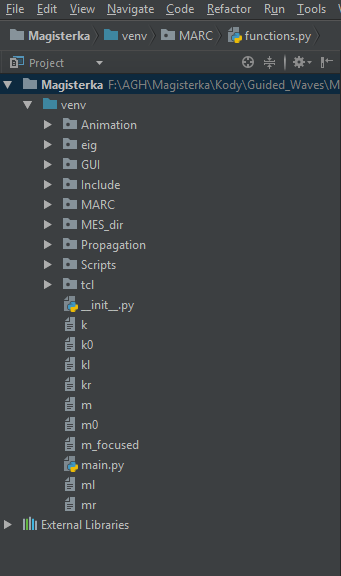
\includegraphics[width=5cm]{Zdjecia/5/okno_projektu}
\caption{Widok okna projektu}
\label{fig:okno_projektu}
\end{figure}

\subsection{Elementy czworościenne}
\label{cha:elementy czworościenne}

Zawartość katalogu MES dir przedstawia rysunek \ref{fig:okno_projektu_MES}. Obliczenia dotyczące elementów czworościennych zawarte są w modułach katalogu tetrahedralElements. Poniżej znajdują się funkcje poszczególnych modułów, wraz z opisem ich zastosowania, argumentami wejściowymi oraz wyjściowymi.

Dane zbierane w postaci macierzy są najczęściej tablicami array z biblioteki NumPy, która służy do obliczeń numreycznych. W części modułów obliczenia są prowadzone na zmiennych symbolicznych z wykorzystaniem biblitoeki SymPy. Macierzy zmiennych symbolicznych są obiektami Matrix z tej biblioteki.

\begin{figure}[h]
\centering
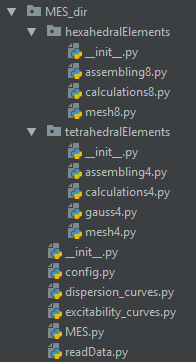
\includegraphics[width=5cm]{Zdjecia/5/okno_projektu_MES}
\caption{Widok okna projektu}
\label{fig:okno_projektu_MES}
\end{figure}


 \( \textbf{Moduł mesh4} \).

\textit{circlePlaneVerticies(x, radius, numberOfPoints)} - funkcja wykorzystywana przy tworzeniu siatki (w circleMeshFull oraz circleMeshSparse). Dodaje do siatki węzły na okręgu w płaszczyźniej pręta na długości x. Promień okręgu określa radius, a ilość węzłów na okręgu to numberOfPoints.

\textit{circleMeshFull(radius, numberOfCircles, numberOfPoints)} - funkcja tworzy siatkę na trzech płaszczyznach przesuniętych o 1 we współrzędnej x. Siatka zbudowana jest na każdej płaszczyźnie tak samo i zawiera węzeł centralny oraz okręgi z węzłami w ilości numberOfCircles. Na każdym okręgu liczba węzłów jest większa, aby zapewnić możliwie równe odległości pomiędzy węzłami. Pierwszy okrąg zawiera liczbę węzłów numberOfPoints. Zwraca tablicę o wymiarach n x 3, gdzie n to liczba węzłów. W kolumnach są kolejne współrzędne węzłów.

\textit{circleMeshSparse(radius, numberOfCircles, numberOfPoints)} - jak wyżej, z tą różnicą, że każdy okrąg siatki ma tyle samo węzłów.

\textit{triangulation(vertices)} - funkcja tworzy elementy skończone czworościenne. Przyjmuje macierz węzłów z powyższych funkcji - vertices i zwraca tablicę e x 4, gdzie e to liczba elementów. W kolumnach zawarte są indeksy węzłów z macierzy wejściowej, które należą do danego elementu.

\textit{correctVolumeSign(vertices, indices)} - funkcja przyjmuje macierz współrzędnych węzłów - vertices oraz indeksy węzłów dla każdego elementu skończonego - indices. Sprawdza czy objętość elementu skończonego obliczona za pomocą wyznacznika ma dodatnią wartość. Jeśli nie, to zmienia miejscami dwa indeksy elementu w macierzy zwróconej z triangulation(vertices).

\textit{drawPlane(vertices)} - funkcja przyjmuje macierz współrzędnych węzłów - vertices i rysuje ich układ na płaszczyźnie. Przykładowe układu przedstawione są na rysunku \ref{fig:siatka}.

\textit{drawBar(vertices)} - funkcja przyjmuje macierz współrzędnych węzłów - vertices i rysuje wszystkie węzły w rzucie izometrycznym. Przykład przedstawia rysunek \ref{fig:pret}.

\textit{drawTriangulation(vertices, indices)} - funkcja przyjmuje macierz współrzędnych węzłów - vertices i macierz elementów skończonych - indices. Rysuje elementy skończone w rzucie izometrycznym. Przykład przedstawia rysunek \ref{fig:triangulation}.

\begin{figure}
\begin{subfigure}{.5\textwidth}
  \centering
  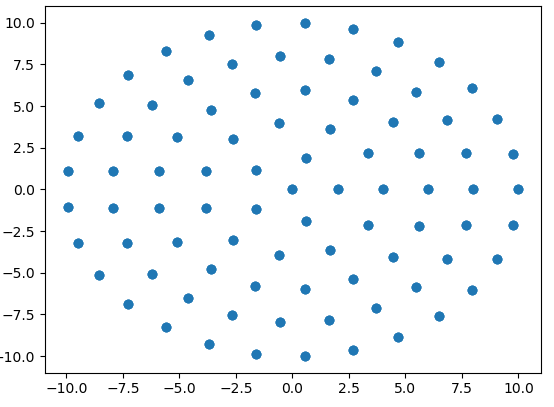
\includegraphics[width=.8\linewidth]{Zdjecia/5/siatka1}
  \caption{}
  \label{fig:sfig1}
\end{subfigure}%
\begin{subfigure}{.5\textwidth}
  \centering
  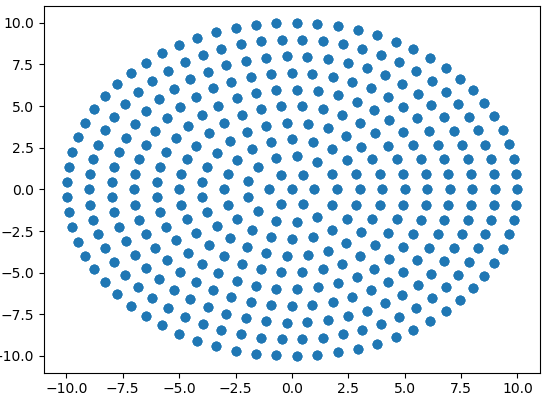
\includegraphics[width=.8\linewidth]{Zdjecia/5/siatka2}
  \caption{}
  \label{fig:sfig2}
\end{subfigure}\\
\begin{subfigure}{.5\textwidth}
  \centering
  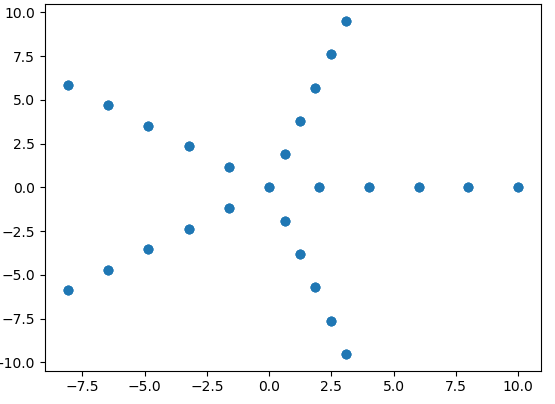
\includegraphics[width=.8\linewidth]{Zdjecia/5/siatka3}
  \caption{}
  \label{fig:sfig3}
\end{subfigure}%
\begin{subfigure}{.5\textwidth}
  \centering
  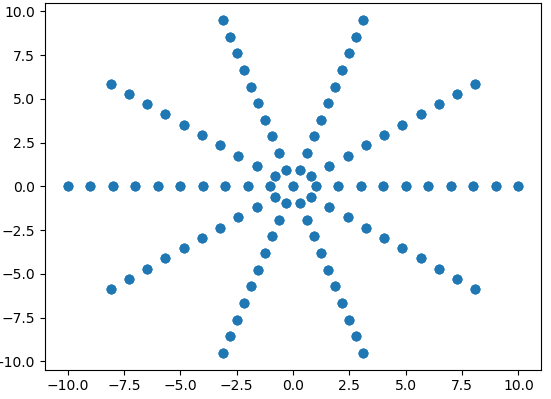
\includegraphics[width=.8\linewidth]{Zdjecia/5/siatka4}
  \caption{}
  \label{fig:sfig4}
\end{subfigure} 
\caption{Układ siatki węzłów na płaszczyźnie powstałych z a) \textit{circleMeshFull(10, 5, 5)} b) \textit{circleMeshFull(10, 10, 10)} c) \textit{circleMeshSparse(10, 10, 10)} d) \textit{circleMeshSparse(10, 10, 10)}}
\label{fig:siatka}
\end{figure}


\begin{figure}
\begin{subfigure}{.5\textwidth}
  \centering
  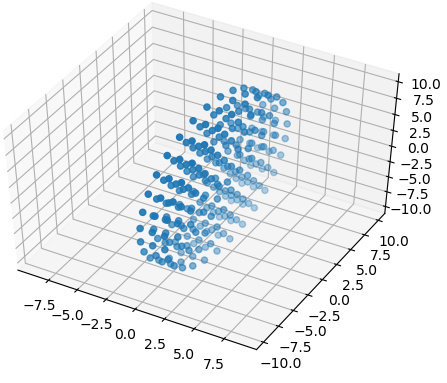
\includegraphics[width=.8\linewidth]{Zdjecia/5/pret1}
  \caption{}
  \label{fig:sfig1}
\end{subfigure}%
\begin{subfigure}{.5\textwidth}
  \centering
  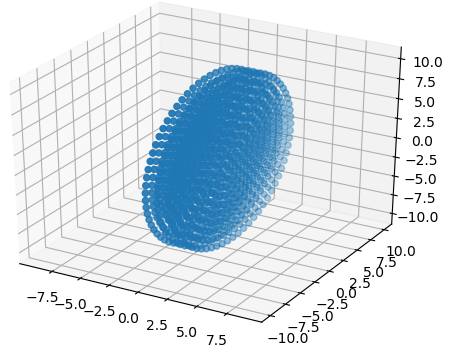
\includegraphics[width=.8\linewidth]{Zdjecia/5/pret2}
  \caption{}
  \label{fig:sfig2}
\end{subfigure}\\
\begin{subfigure}{.5\textwidth}
  \centering
  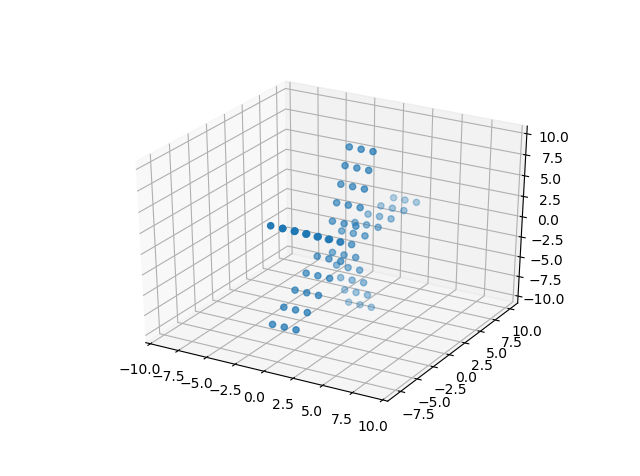
\includegraphics[width=.8\linewidth]{Zdjecia/5/pret3}
  \caption{}
  \label{fig:sfig3}
\end{subfigure}%
\begin{subfigure}{.5\textwidth}
  \centering
  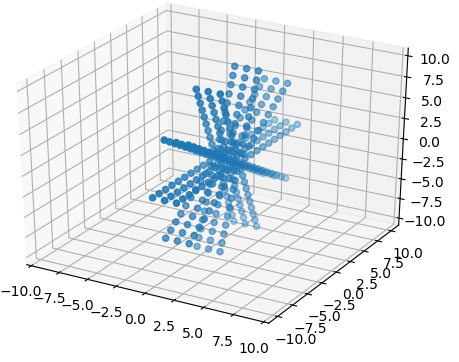
\includegraphics[width=.8\linewidth]{Zdjecia/5/pret4}
  \caption{}
  \label{fig:sfig4}
\end{subfigure} 
\caption{Układ siatki węzłów pręta z a) \textit{circleMeshFull(10, 5, 5)} b) \textit{circleMeshFull(10, 10, 10)} c) \textit{circleMeshSparse(10, 10, 10)} d) \textit{circleMeshSparse(10, 10, 10)}}
\label{fig:pret}
\end{figure}

\begin{figure}
\begin{subfigure}{.5\textwidth}
  \centering
  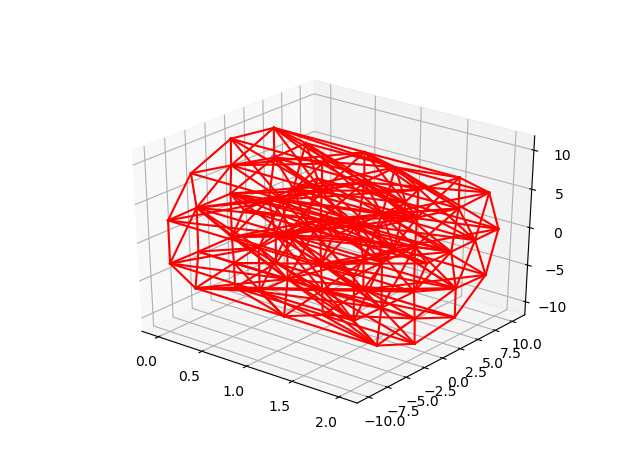
\includegraphics[width=.8\linewidth]{Zdjecia/5/triangulation1}
  \caption{}
  \label{fig:sfig1}
\end{subfigure}%
\begin{subfigure}{.5\textwidth}
  \centering
  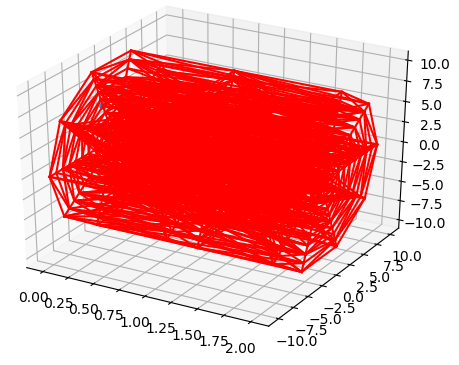
\includegraphics[width=.8\linewidth]{Zdjecia/5/triangulation2}
  \caption{}
  \label{fig:sfig2}
\end{subfigure}

\caption{Triangulacja (elementy skończone) dla siatki a) \textit{circleMeshFull(10, 3, 3)} b) \textit{circleMeshSparse(10, 10, 10)}}
\label{fig:triangulation}
\end{figure}

 \( \textbf{Moduł calculation4} \).

\textit{pVector()} - funkcja zwraca macierz zmiennych symbolicznych z wektorem p dla elementu czworościennego.

\textit{meMatrix(vertices, elementIndices)} - funkcja przyjmuje macierz współrzędnych węzłów - vertices oraz indeksy dla węzłów elementu skończonego - elementIndices i zwraca macierz \( M^e \).

\textit{meInvMatrix(vertices, elementIndices)} - jak powyżej, dodatkowo odwraca macierz wyjściową.

\textit{shapeFunctions(vertices, elementIndices)} - funkcja przyjmuje macierz współrzędnych węzłów - vertices i indeksy dla węzłów elementu skończonego - elementIndices, a zwraca funkcje kształtu w formie tablicy zmiennych symbolicznych.

\textit{bMatrixFc(shapeFunctions)} - funkcja przyjmuje tablicę funkcji kształtu w postaci symbolicznej - shapeFunctions, a zwraca macierz B w postaci tablicy numerycznej. Funkcje kształtu są dla elementów czworościennych liniowe więc ich pochodne są stałymi. 

\textit{bMatrixNatural(shapeFunctions)} - jak powyżej, ale dla tablicy funkcji kształtu we współrzędnych naturalnych.

\textit{dMatrixFc(youngModulus, poissonCoeficient)} - funkcja zwraca macierz D, obliczoną na podstawie modułu Younga - youngModulus oraz współczynnik Poissona - poissonCoeficient.

\textit{stiffLocalMatrix(shapeFunctions, vertices, elementIndices, youngModulus, poissonCoefficient)} - funkcja przyjmuje jako argumenty funkcje kształtu w formie symbolicznej - shapeFunctions, macierz współrzędnych węzłów - vertices, indeksy węzłów elementu skończonego - element indices oraz moduł Younga - youngModulus i współczynnik Poissona - poissonCoeficient. Zwraca macierz sztywności dla elementu skończonego.

\textit{massLocalMatrix(density)} - funkcja przyjmuje gęstość materiału - density. Zwraca macierz mas obliczoną we współrzędnych naturalnych bez uwzględnienia jakobianu. Na tym etapie nie jest to więc poprawnie wyznaczona macierz mas. Jakobian jest stały dla elementów czworościennych i uwzględniany jest na etapie agregacji. Pozwala to obliczyć całkę \ref{} raz, a następnie mnożyć ją dla każdego elementu przez jakobian.

\textit{volume(elementVertices)} - funkcja przyjmuje współrzędnych węzłów elementu - elementVertices i oblicza objętość elementu z wykorzystaniem geometrii analitycznej.

\textit{volumeDet(vertices)} - jak powyżej z tym, że objętość jest obliczano za pomocą wyznacznika macierzy \( M^e \).

 \( \textbf{Moduł gauss4} \).
Moduł zawiera funkcje pomocnicze do całkowania macierzy mas. Obliczanie macierzy sztywności nie wymaga całkowania, ponieważ macierz B jest stała.

\textit{shapeFunctionsNatural()} - zwraca tablicę funkcji kształtu we współrzędnych naturalnych, w formie symbolicznej.

\textit{coordinateChangeModel(elementVertices, naturalShapeFc)} - funkcja przyjmuje funkcje kształtu we współrzędnych naturalnych - naturalShapeFc  oraz współrzędne węzłów elementu skończonego - elementVertices i oblicza zależność współrzędnych rzeczywistych i naturalnych. Zwraca trzy wyrażenia symboliczne zawierające współrzędne naturalne. Przedtsawiają one współrzędne rzeczywiste, kolejno x, y, z.

\textit{jacobian(elementVertices, naturalShapeFc)} - funkcja przyjmuje współrzędne węzłów elementu skończonego - elementVertices oraz funkcje kształtu we współrzędnych naturalnych - naturalShapeFc. Zwraca jakobian przekształcenia, który jest wykorzystywany w obliczaniu macierzy mas.

\textit{matrixToIntegrate(density)} - funkcja przyjmuje gęstość materiału - density. Zwraca macierz podcałkową, do obliczania macierzy mas. Nie uwzględnia jakobianu, który jest stały. Wynik całkowania jest mnożony przez jakobian na etapie agregacji.

 \( \textbf{Moduł assembling4} \).
Moduł zawiera funkcje do obliczania macierzy globalnych. Pozwala też na wizualizację rzadkości macierzy.

\textit{assembleGlobalStiffMatrix(vertices, indices, youngModulus, poissonCoefficient)} - funkcja przyjmuje macierz współrzędnych węzłów konstrukcji - vertices, indeksy wszystkich elementów - indices, moduł Younga - youngModulus i współczynnik Poissona - poissonCoeficient. Zwraca globalną macierz sztywności.

\textit{drawMatrixSparsity(matrix)} - funkcja przyjmuje macierz - matrix. Pozwala rysować rzadkość macierzy w postaci bitmapy, gdzie każdy element macierzy jest jednym pikselem.

\textit{assembleGlobalMassMatrix(vertices, indices, density)} - funkcja przyjmuje macierz współrzędnych węzłów konstrukcji - vertices, indeksy wszystkich elementów skończonych - indices oraz gęstość materiału - density. Zwraca globalną macierz mas.

\textit{focuseMatrixRows(matrix)} - funkcja przyjmuje macierz - matrix. Zwraca macierz skupioną poprzez sumowanie elementów w wierszu i umieszczanie ich na diagonali. Wykorzystywana przy obliczeniach ze skupioną macierza mas.

\subsection{Elementy sześcienne}
\label{cha:elementy szescienne}

Obliczenia dotyczące elementów sześciennych zawarte są w modułach katalogu hexahedralElements. Poniżej znajdują się funkcje poszczególnych modułów, wraz z opisem ich zastosowania, argumentami wejściowymi oraz wyjściowymi.

 \( \textbf{Moduł mesh8} \).

\textit{circleMeshFull(radius, firstCircle, addNodes, circles)} - funkcja działa jak funcja z modułu mesh4 z tą różnicą, że przyjmuje dodatkowy argument addNodes. Określa on ile punktów więcej ma być na każdym kolejnym okręgu siatki.

\textit{circleMeshSparse(radius, firstCircle, circles)} - funkcja działa jak odpowiednik z modułu mesh4

\textit{createFiniteElements(vertices, pointsOnLastCircle, length, numberOfPlanes)} - funkcja przyjmuje jako argumenty macierz współrzędnych węzłów, liczbę punktów na ostatnim okręgu siatki, długość modelu pręta oraz liczbę płaszczyzn siatki. Tworzy elementy sześcienne w kilku etapach. Najpierw jedna z płaszczyzn dzielona jest na trójkąty. Następnie trójkąty są łączone w pary i w ten sposób powstają czworokąty. W większości konfiguracji siatki na brzegach pozostają puste miejsca z trójkątów, które nie mają pary. W takich miejscach dodawany jest dodatkowy punkt siatki i z trójkąta tworzony czworokąt. Następnie identyczne czworokąty są tworzone na kolejnych płaszczyznach i wzdłuż długości pręta tworzone są z nich sześciościany. Zwraca macierz e x 8, gdzie e to liczba elementów skończonych. W kolumnach są indeksy kolejnych punktów siatki.

\textit{brickMesh(radius, numberOfPlanes, numberOfCircles, numberOfPointsOnCircle)} - funkcja tworzy siatkę w kształcie wielokąta. Przyjmuje jako argumenty promień - radius, liczbę płaszczyzn siatki - numberOfPlanes, liczbę okręgów na płaszczyźnie siatki - numberOfCircles oraz ilość wierzchołków wielokąta wpisanego w okrąg - numberOfPointsOnCircle. Zwraca tablicę o wymiarach n x 3, gdzie n to liczba węzłów. W kolumnach są kolejne współrzędne węzłów.

\textit{createBrickElements(brickVertices, numberOfPlanes, numberOfCircles, numberOfPointsOnCircle)} - funkcja przyjmuje macierz współrzędnych węzłów z funkcji \textit{brickMesh} - brickVertices, liczbę płaszczyzn siatki - numberOfPlanes, liczbę okręgów na każdej płaszczyźnie - numberOfCircles oraz liczbę wierzchołków wielokąta wpisanego w każdy okrąg - numberOfPointsOnCircle. Tworzy elementy sześciościenne na zadanej siatce. Zwraca macierz e x 8, gdzie e to liczba elementów skończonych. W kolumnach są indeksy kolejnych punktów siatki.

\textit{drawPlane(vertices)} - jak w mesh4. Przykładowe siatki z tego modułu są przedstawione na rysunku \ref{}.

\textit{drawBar(vertices)} - jak w mesh4

\textit{drawTetragons(vertices, indices)} - funkcja przyjmuje jako argumenty macierz współrzędnych węzłów - vertices oraz macierz indeksów węzłów dla każdego elementu - indices. Rysuje układ czworokątów na płaszczyźnie. Przykłady są przedstawione na rysunku r\ref{}.

\textit{drawHexahedrons(vertices, indices)} - funkcja przyjmuje jako argumenty macierz współrzędnych węzłów - vertices oraz macierz indeksów węzłów dla każdego elementu - indices. Rysuje model złożony z sześciościanów w rzucie izometrycznym.
